\documentclass[smaller,pdf,svgnames]{beamer}

\usepackage{color}
\usepackage{dsfont}

\useinnertheme{circles}

\title {Heteroscedastic Linear Discriminant Analysis}
\author[Thomas Badie \and Gary Perelman \and Pierre Parutto]{Thomas Badie\\Gary Perelman\\Pierre Parutto}

\usetheme{Warsaw}

\usecolortheme[rgb={.6,0,.6}]{structure}

%% To get the page numbering clean.
\defbeamertemplate*{footline}{shadow theme}
{%
  \leavevmode%
  \hbox{\begin{beamercolorbox}[wd=.5\paperwidth,ht=2.5ex,dp=1.125ex,leftskip=.3cm plus1fil,rightskip=.3cm]{author in head/foot}%
    \usebeamerfont{author in head/foot}\insertframenumber\,/\,\inserttotalframenumber\hfill\insertshortauthor
  \end{beamercolorbox}%
  \begin{beamercolorbox}[wd=.5\paperwidth,ht=2.5ex,dp=1.125ex,leftskip=.3cm,rightskip=.3cm plus1fil]{title in head/foot}%
    \usebeamerfont{title in head/foot}\insertshorttitle%
  \end{beamercolorbox}}%
  \vskip0pt%
}

% To do not have the summary on each slide.
\setbeamertemplate{headline}{}

\begin{document}

\begin{frame}
  \maketitle
\end{frame}

\begin{frame}{Table of contents}
  \tableofcontents
\end{frame}

\section{From LDA to HLDA}

\subsection{Quick LDA review}

\begin{frame}
  \frametitle{Linear Discriminant Analysis}

  \begin{block}{Multi-class LDA}
    \begin{itemize}
    \item Definition based on \cite{bishop2006pattern}
    \item Find the linear transformation $A$
    \item Minimize the within-class covariance $S_W$
    \item Maximize the between-class covariance $S_B$
    \end{itemize}
  \end{block}

  \begin{block}{Equations}
    $$\begin{array}{ccl}
      S_B & = & \frac{1}{C} \times \sum\limits_{i = 1}^C (\mu_i - \mu)(\mu_i - \mu)^t \\
      S_W & = & \frac{1}{C} \times \sum\limits_{i = 1}^C \sum\limits_{\forall x \in C_i} (x - \mu_i)(x - \mu_i)^t\\
      A & = & {S_W}^{-1} S_B
    \end{array}$$
  \end{block}
\end{frame}

\subsection{Limitations}

\begin{frame}
  \begin{block}{LDA's limitation}
    \begin{itemize}
      \item LDA assumes the homoscedastic class covariance
      \item Differences between classes must lie in their mean
    \end{itemize}
  \end{block}

  \centering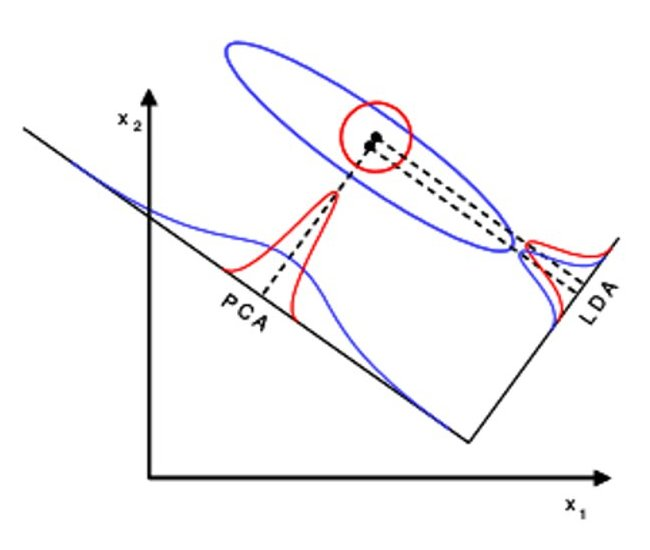
\includegraphics[scale=0.4]{../img/limitation_lda}

\end{frame}

\section{HLDA method}

\subsection{Presentation}

\begin{frame}
  \begin{block}{hypothesis}
    \begin{itemize}
    \item Developed by Kumar \cite{kumar.1997}
    \item The space can be divided into two subspaces of size $p$ and $n-p$ with $p < n$
    \item The space of size $p$ bear the class dependent information
    \item The space of size $n-p$ is common to all classes
    \end{itemize}
  \end{block}

  \begin{block}{Goal}
    \begin{itemize}
      \item Find the linear transformation $A$
      \item
        $$A = \left [
          \begin{array}{c}
            A_p\\
            A_{n-p}
          \end{array}
        \right ]
        $$
      \item $A_p$ is the final projection matrix (hence the dimension reduction)
    \end{itemize}
  \end{block}
\end{frame}

\begin{frame}
  \frametitle{Maximum likelihood}

  \begin{block}{HLDA Gaussian model}
    $$P(y_i) = \frac{\mid \theta \mid}{\sqrt{(2\pi)^n \mid \Sigma_{g(i)} \mid}}
    e^{-\frac{1}{2} (y_i - \mu_{g(i)})^t \Sigma_{g(i)}^{-1} (y_i - \mu_{g(i)})}$$
  \end{block}

  \begin{block}{Maximum likelihood}
    \begin{itemize}
      \item No analytical solution
      \item Parameters : $\mu_j$, $\Sigma_j$ and $A$
      \item Different equations depending on the type of $\Sigma_j^p$
    \end{itemize}
  \end{block}

\end{frame}

\begin{frame}
  \frametitle{Resolution for a diagonal $\Sigma_j^p$}

  \begin{block}{ML equation for a diagonal $\Sigma_j^p$}
    $$
    \begin{array}{cl}
      Log L_D(\mu_j, \Sigma_j, A; \{x_i\}) = & -\frac{N n}{2} Log (2\pi) + N Log|A| - \frac{N}{2}\sum\limits_{k = p + 1}^n Log|\sigma^k| \\
      & - \sum\limits_{j = 1}^J \frac{N_j}{2} \sum\limits_{k = 1}^p Log|\sigma_j^k| - \frac{1}{2}\sum\limits_{j = 1}^J\sum\limits_{g(i) = j}
      \sum\limits_{k = 1}^p \frac{(\vec{A_k^T} - \mu_{j,k})^2}{\sigma_j^k} \\
      & + \frac{1}{2}\sum\limits_{j = 1}^J\sum\limits_{g(i) = j}
      \sum\limits_{k = p + 1}^p \frac{(\vec{A_k^T} - \mu_{0,k})^2}{\sigma^k}
    \end{array}
    $$
  \end{block}

  \begin{block}{Finding $\mu_j^p$ and $\Sigma_j^p$}
    $$
    \begin{array}{ccl}
      \frac{\partial Log L_D(\mu_j, \Sigma_j, A; \{x_i\})}{\partial \mu_j} & \Rightarrow & \left \{
        \begin{array}{ccl}
          \hat\mu_j^p & = & A_p^T\bar{X_j} ,\; j = 1...J\\
          \hat\mu_0 & = & A_{n - p}^T\bar{X}
        \end{array}
      \right . \\
      \frac{\partial Log L_D(\mu_j, \Sigma_j, A; \{x_i\})}{\partial \Sigma_j} & \Rightarrow & \left \{
        \begin{array}{ccl}
          \hat\Sigma_j^p & = & Diag(A_p^T\bar{W_j}A_p), \; j = 1...J\\
          \hat\Sigma^{n - p} & = & Diag(A_{n - p}^T\bar{T}A_{n - p})
        \end{array}
      \right .
    \end{array}
    $$
  \end{block}
\end{frame}

\subsection{Numerical approximation}

\begin{frame}
  \frametitle{Numerical approximation}

  \begin{block}{Method}
    \begin{itemize}
      \item There are no analytical solutions for $\hat{A_F}$ and $\hat{A_D}$
      \item Must use a numerical-optimization method
      \item Any such method may be used
      \item Kumar\cite{kumar.1997} uses a Gradient descent algorithm
    \end{itemize}
  \end{block}
\end{frame}

\section{Benchmarks}

\subsection{Setup}

\begin{frame}
  \frametitle{Environment}

  \begin{block}{Database}
    \begin{itemize}
      \item MNIST database
      \item $28 \times 28$ pixels images representing digits from $0$ to $9$
      \item $10$ corresponding classes
    \end{itemize}
  \end{block}

  \begin{block}{Method}
    \begin{itemize}
      \item Nearest mean classifier used
      \item because of memory consumption a PCA is applied on the samples keeping only 250 dimensions
      \item Matlab implementation found in \cite{burget.2004}
    \end{itemize}
  \end{block}

\end{frame}

\subsection{Results}

\begin{frame}
  \frametitle{Number of dimensions kept}
  \centering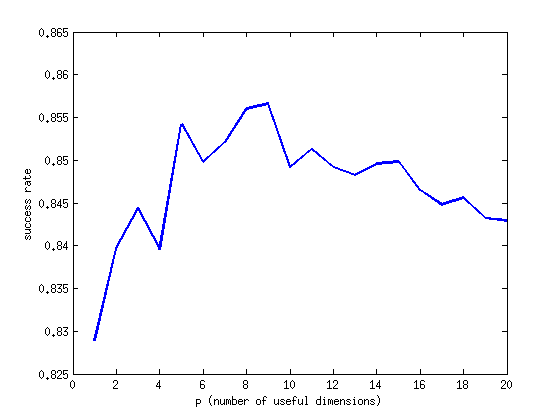
\includegraphics[scale=0.70]{../img/bench-classes}
\end{frame}

\begin{frame}
  \frametitle{Convergence issue}
  \centering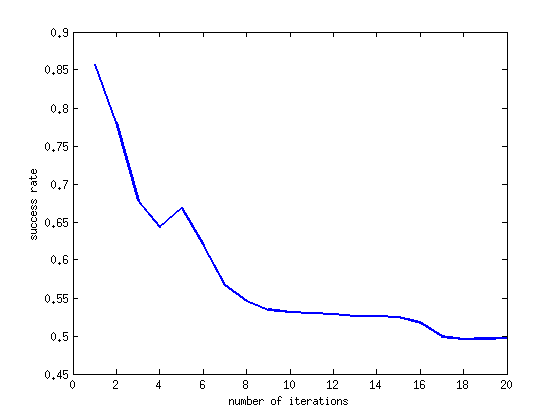
\includegraphics[scale=0.70]{../img/bench-iterations}
\end{frame}

\begin{frame}
  \frametitle{Points separation}
  \centering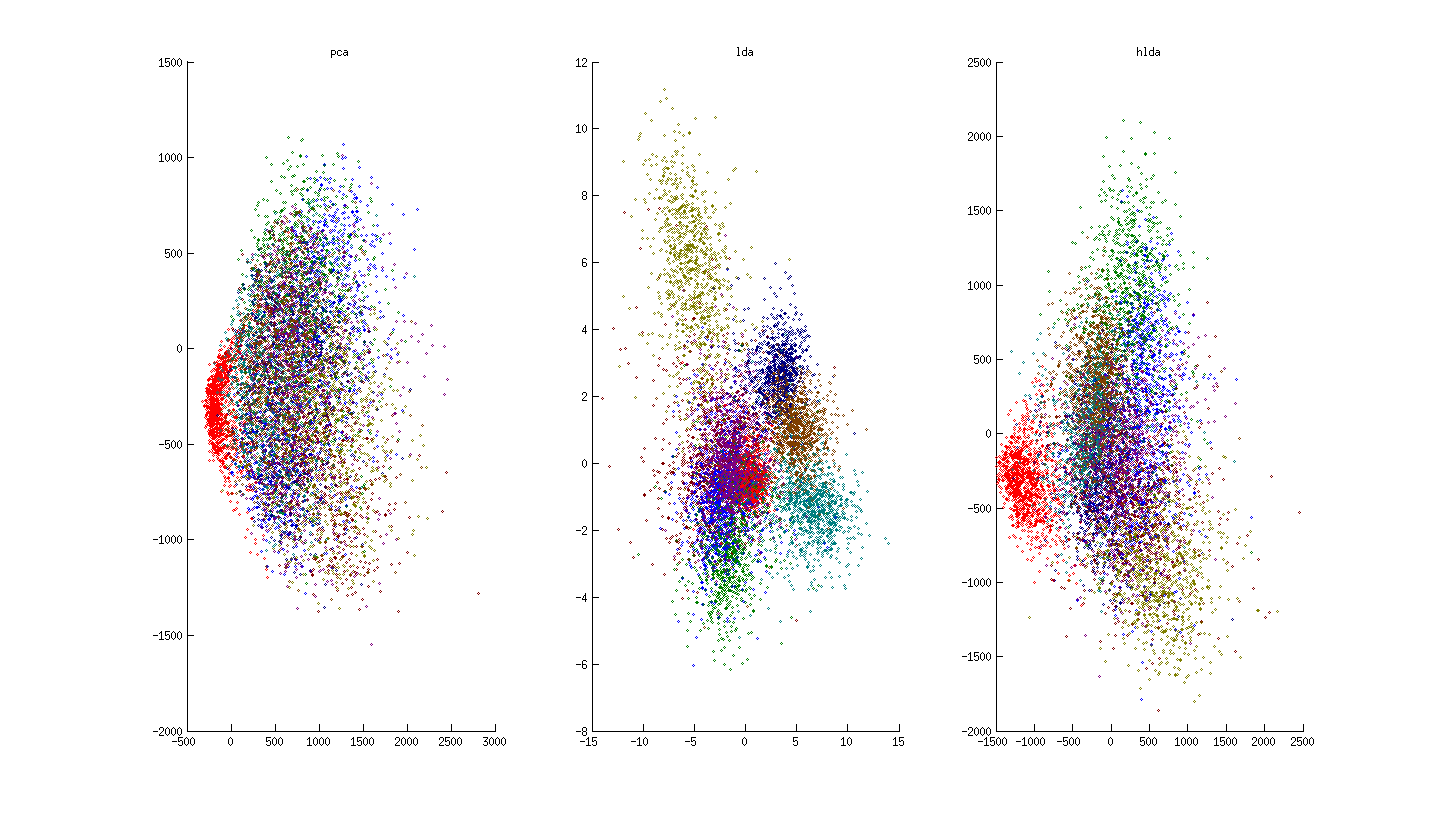
\includegraphics[scale=0.30]{../img/classif}
\end{frame}

\section{Conclusion}

\begin{frame}
  \frametitle{Conclusion}

  \begin{block}{On the method}
    \begin{itemize}
    \item HLDA allows a better classification for heteroscedastic classes
    \item Uses the maximum-likelihood method
    \item No analytical solutions
    \item Must use numerical approximation methods
    \end{itemize}
  \end{block}

  \begin{block}{On the implementation}
    \begin{itemize}
    \item Did not obtain better result on the MNIST database
    \item May be due to wrong parameters for the algorithm
    \item Takes a lot of time to compute (compared to the LDA)
    \end{itemize}
  \end{block}

  \begin{block}{Related methods}
    \begin{itemize}
      \item BDHLDA, based on block decomposition presented in \cite{zhang2011}
      \item SHLDA, for small training dataset, presented in \cite{burget.2004}
    \end{itemize}
  \end{block}
\end{frame}

\begin{frame}
  \frametitle{Questions?}
\end{frame}

\section{References}

\begin{frame}[allowframebreaks]{Bibliography}
  \footnotesize
  \bibliographystyle{unsrt}
  \bibliography{../biblio}
\end{frame}

\end{document}
